%==============================================================
This chapter presents design examples of each chip in the MCS-4 system—namely, the 4004 (CPU), 4001 (ROM), 4002 (RAM), and 4003 (Shift Register)—implemented using Verilog HDL.

The RTL descriptions for each MCS-4 chip are stored in the directory \texttt{RTL/MCS4/}.
%==============================================================
\section{Differences Between Physical Chip Design and RTL Design}
In this project, each chip of the MCS-4 system is implemented with equivalent functionality using Verilog HDL and deployed onto an FPGA. However, due to the legacy nature of the original chip design, the following modifications were necessary:

\begin{itemize}
  \item \textbf{System Clock:}  
  The original chips employ a latch-based design and utilize a two-phase non-overlapping clock system. In contrast, the FPGA implementation adopts D flip-flop–based circuits synchronized with the rising edge of the clock, using a single-phase clock.

  \item \textbf{Data Bus:}  
  The 4004 (CPU), 4001 (ROM), and 4002 (RAM) chips feature a 4-bit bidirectional data bus. When integrating these chips into a single FPGA, bidirectional buses cannot be directly implemented. Therefore, the data bus \texttt{DATA[3:0]} is divided into an input bus \texttt{DATA\_I[3:0]} and an output bus \texttt{DATA\_O[3:0]}, along with an output enable signal \texttt{DATA\_OE} to indicate when the output bus is active.

  \item \textbf{External Data Bus Connection:}  
  If the data bus is routed to an external device outside the FPGA, it will be configured as a bidirectional bus. To prevent signal contention, it is driven in open-drain mode and internally equipped with a pull-up resistor within the FPGA.
\end{itemize}
%==============================================================
\section{Internal States of MCS-4 Chips and System Synchronization}
In the MCS-4 system, all chips—including the 4004 (CPU), 4001 (ROM), and 4002 (RAM)—must operate in synchronization. The CPU has eight internal states:

\begin{itemize}
  \item A1, A2, A3
  \item M1, M2
  \item X1, X2, X3
\end{itemize}

It is essential that the internal state of each chip remains fully synchronized with the CPU.
%--------------------------------------------------------------
\subsection{State Signal Definition}
To represent internal states, an 8-bit signal \verb|state[7:0]| is defined. Each of the eight bits corresponds to a specific state. For example:

\begin{itemize}
  \item A1: \verb|8'b0000_0001|
  \item X3: \verb|8'b1000_0000|
\end{itemize}

At no time are multiple bits set simultaneously.
Each chip (CPU, ROM, and RAM) shares the same \verb|state[7:0]| signal, which must be synchronized across the system.

%--------------------------------------------------------------
\subsection{System Synchronization Using \texttt{sync\_n}}
The method of synchronizing internal states is illustrated in Figure~\ref{fig:SYNC-METHOD}. The system synchronization signal \verb|sync_n| is used.

Figure~\ref{fig:SYNC-METHOD} shows the transition from system reset to the beginning of CPU instruction execution. During reset, \verb|state[7:0]| is cleared to all zeros.

At the rising edge of the first clock after reset is released:
\begin{itemize}
  \item CPU sets \verb|state_next[7:0]| to A1
  \item \verb|sync_n| is asserted
\end{itemize}

Afterward, the CPU sequentially updates \verb|state_next[7:0]| and transfers it to \verb|state[7:0]| on each rising clock edge, advancing the internal state.

On the ROM/RAM side:
\begin{itemize}
  \item When \verb|sync_n| is asserted at the clock’s rising edge, \verb|state[7:0]| is set to A1
  \item Then the internal states progress in sync with the CPU
\end{itemize}

This ensures all chips start execution in a synchronized manner.

%--------------------------------------------------------------
\begin{figure}[h]
  \centering
  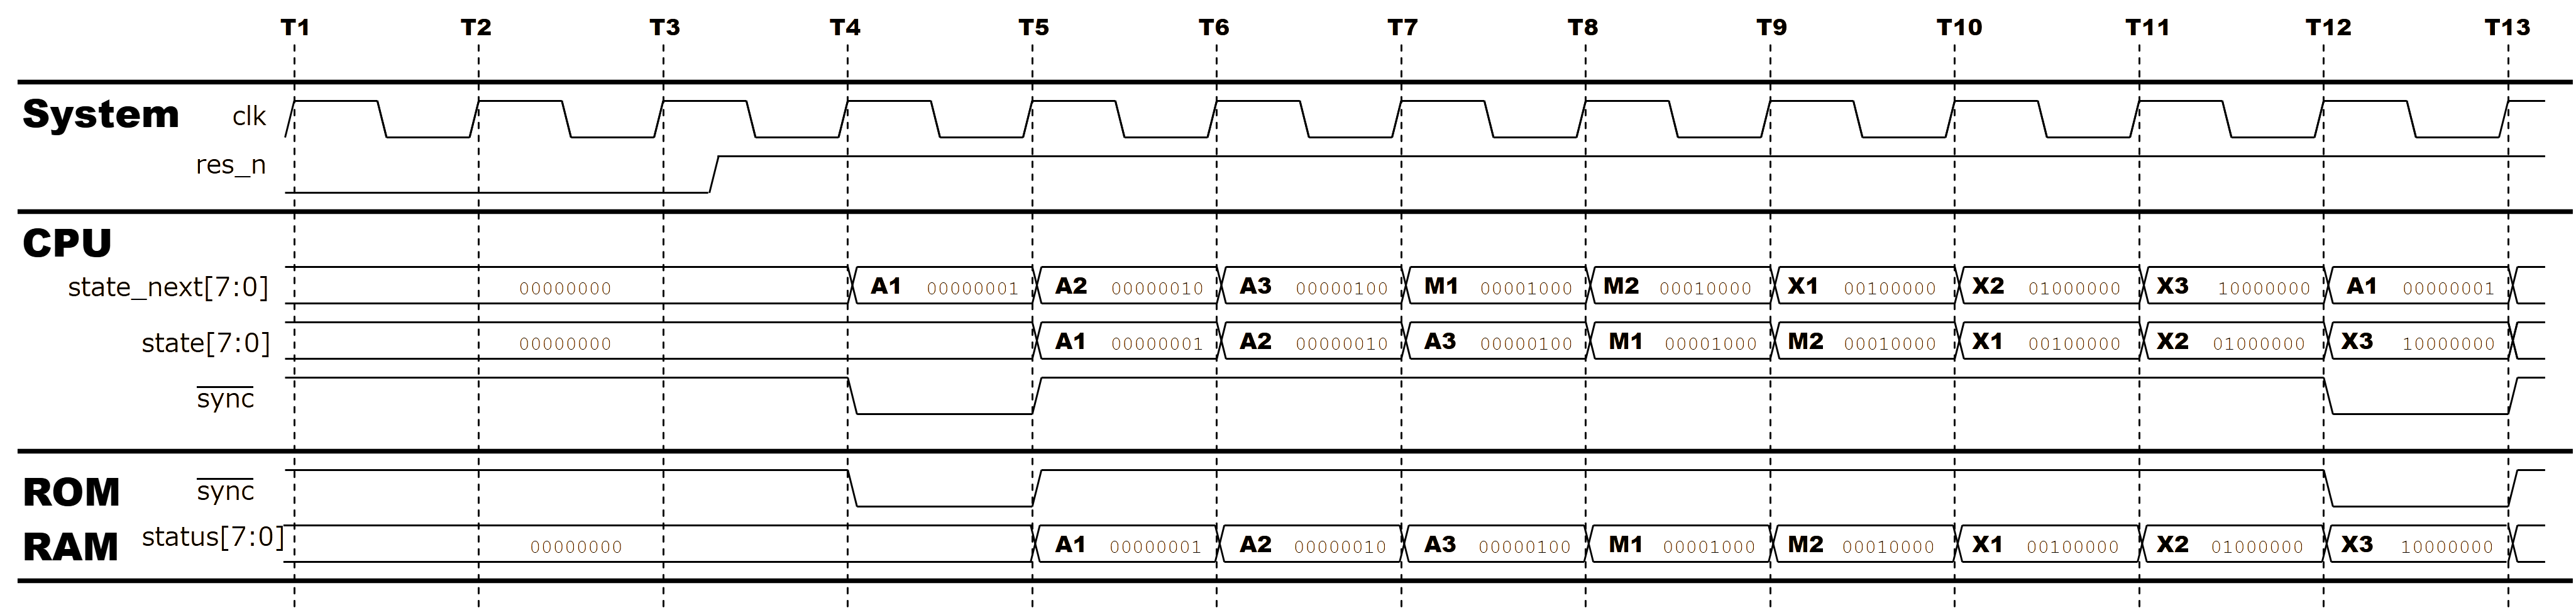
\includegraphics[width=1.0\textwidth]{./Figure/SyncMethod.png}
  \caption{System synchronization method using \texttt{SYNC} signal}
  \label{fig:SYNC-METHOD}
\end{figure}
%--------------------------------------------------------------
%==============================================================
\section{Logic of the \texttt{MCS4\_CPU} Module (4004)}
The entire CPU datapath and control unit are described within the RTL code file \texttt{mcs4\_cpu.v}. The implementation is compact, consisting of fewer than 1000 lines, including comments. The code is written with readability in mind, allowing for a clear understanding of its structure and behavior from the RTL alone. 
Table~\ref{tb:SIGNALSMCS4CPU} lists the input and output signals of the \texttt{MCS4\_CPU} module.
Below is a brief explanation of each major section of the CPU design.

%----------------------------------
\begin{table}[htbp]
    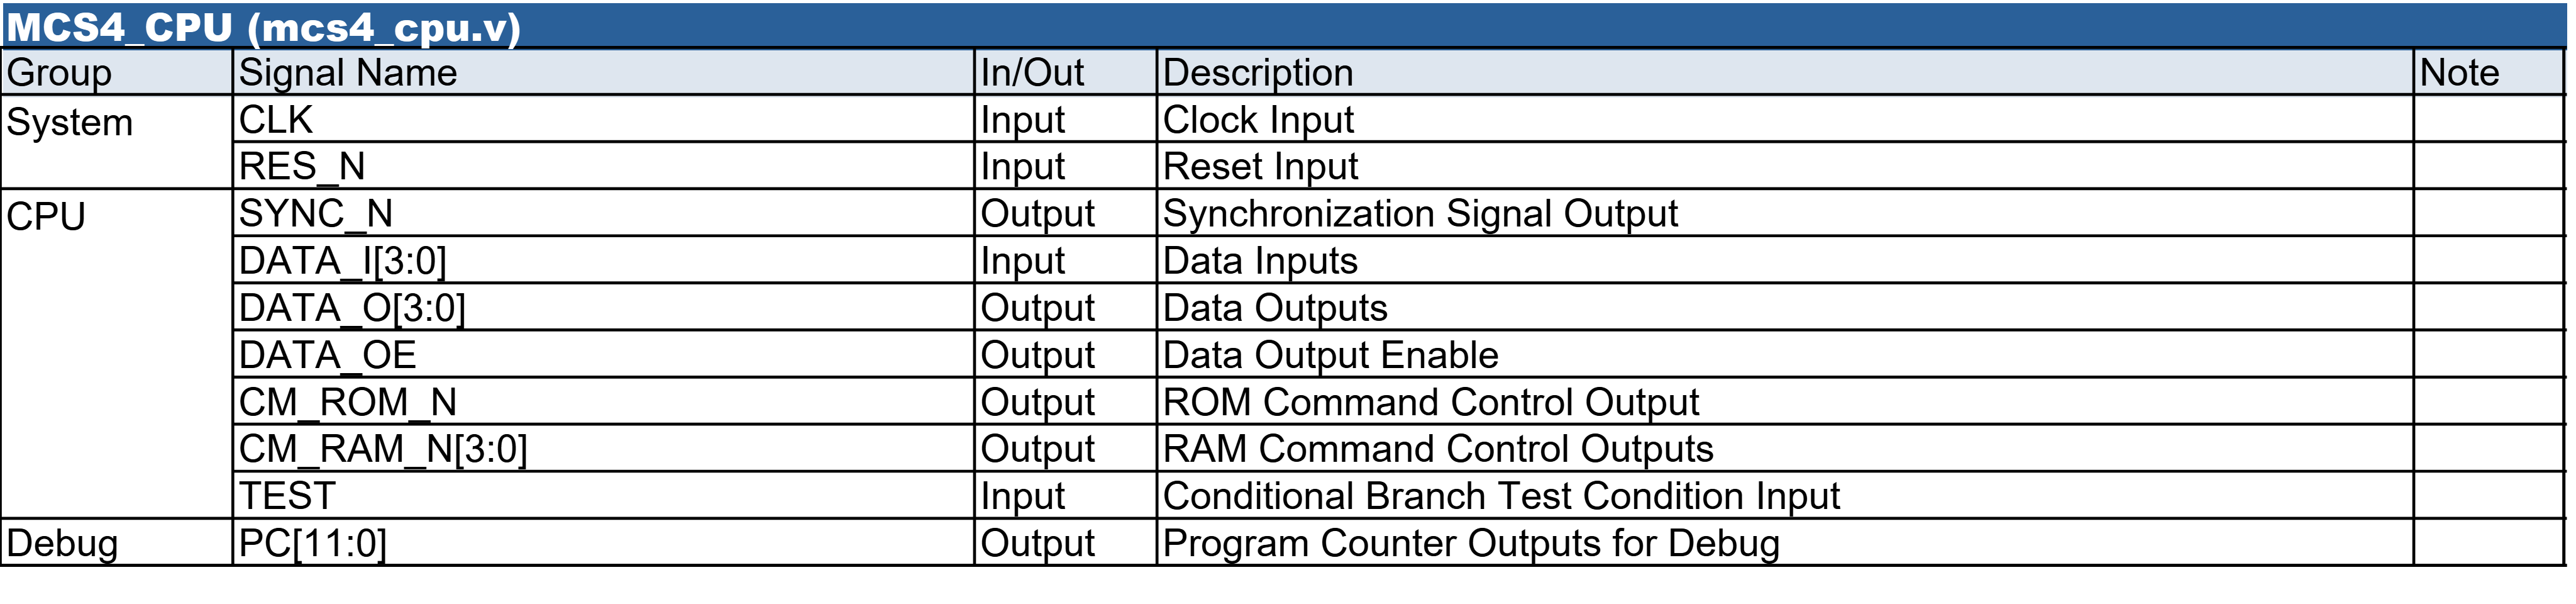
\includegraphics[width=1.00\columnwidth]{./Table/SignalsMCS4CPU.png}
    \caption{I/O Signals of \texttt{MCS4\_CPU}}
    \label{tb:SIGNALSMCS4CPU}
\end{table}
%----------------------------------

%--------------------------------------------------------------
\begin{enumerate}[(1)]
%--------------------------------------------------------------
\item \textbf{Definition of System State}\\
\begin{lstlisting}[caption=Definition of System State, 
label=list:MCS4CPU01, captionpos=b,  language=, frame=single, basicstyle=\ttfamily\scriptsize]
//---------------
// State Number
//---------------
`define A1 0
`define A2 1
`define A3 2
`define M1 3
`define M2 4
`define X1 5
`define X2 6
`define X3 7
\end{lstlisting}

%--------------------------------------------------------------
\item \textbf{Definition of input/output signals and internal signals}\\
The 12-bit wide program counter (PC) is exposed externally to drive the LED indicators on the FPGA board.\\
\begin{lstlisting}[caption=Definition of input/output signals and internal signals, 
label=list:MCS4CPU02, captionpos=b,  language=, frame=single, basicstyle=\ttfamily\scriptsize]
//======================================
// Module : CPU Core
//======================================
module MCS4_CPU
(
    input  wire       CLK,      // clock
    input  wire       RES_N,    // reset_n
    //
    output wire       SYNC_N,   // Sync Signal
    input  wire [3:0] DATA_I,   // Data Input
    output wire [3:0] DATA_O,   // Data Output
    output wire       DATA_OE,  // Data Output Enable
    output wire       CM_ROM_N, // Memory Control for ROM
    output wire [3:0] CM_RAM_N, // Memory Control for RAM
    input  wire       TEST,     // Test Input
    //
    output wire [11:0] PC  // debug
);

integer i;

//--------------------
// Main CPU Resource
//--------------------
wire [11:0] pc;      // Program Counter
wire [11:0] pc_next; // Next PC
reg  [ 3:0] acc;     // Accumulator
reg         cy;      // Carry Borrow Flag
reg  [ 3:0] r[0:15]; // Index Registers
wire [ 3:0] rn;      // Index Register specified by opropa0
wire [ 7:0] rp;      // Index Register Pair specified by opropa0
reg  [ 2:0] dcl;     // Designate Comand Line
reg  [ 7:0] src;     // Send Register Control

assign PC = pc;
\end{lstlisting}

%--------------------------------------------------------------
\item \textbf{Control of Internal State Transitions}\\
\begin{lstlisting}[caption=Control of Internal State Transitions, 
label=list:MCS4CPU03, captionpos=b,  language=, frame=single, basicstyle=\ttfamily\scriptsize]
//---------------------------------
// State Count
//---------------------------------
reg  [7:0] state;
reg  [7:0] state_next;
reg        multi_cycle;
reg        multi_cycle_inc;
//
always @(posedge CLK, negedge RES_N)
begin
    if (~RES_N)
        state <= 8'b00000000;
    else
        state <= state_next;
end
//
always @*
begin
    casez(state)
        8'b00000000 : state_next = 8'b00000001;
        8'b10000000 : state_next = 8'b00000001;
        default     : state_next = {state[6:0], state[7]}; // rotate left
    endcase
end
\end{lstlisting}

%--------------------------------------------------------------
\item \textbf{Control for multi-cycle instructions}\\
The following describes the control for multi-cycle instructions requiring two instruction cycles. During the first cycle, \verb|multi_cycle| is \verb|1'b0|; in the second, it becomes \verb|1'b1|. 
\\
\begin{lstlisting}[caption=Control for multi-cycle instructions, 
label=list:MCS4CPU04, captionpos=b,  language=, frame=single, basicstyle=\ttfamily\scriptsize]
//----------------------------------
// Control of 2-Cycle Instruction
//----------------------------------
always @(posedge CLK, negedge RES_N)
begin
    if (~RES_N)
        multi_cycle <= 1'b0;
    else if (multi_cycle_inc)
        multi_cycle <= ~multi_cycle;
end
\end{lstlisting}

%--------------------------------------------------------------
\item \textbf{Generation of the \texttt{sync\_n} signal}\\
\begin{lstlisting}[caption=Generation of the \texttt{sync\_n} signal, 
label=list:MCS4CPU05, captionpos=b,  language=, frame=single, basicstyle=\ttfamily\scriptsize]
//------------------------
// Generate Sync Signal
//------------------------
assign SYNC_N = ~state_next[`A1];
\end{lstlisting}

%--------------------------------------------------------------
\item \textbf{Program Counter (PC) and the Stack (Program Address Register)}\\
\begin{lstlisting}[caption=Program Counter (PC) and the Stack (Program Address Register), 
label=list:MCS4CPU06, captionpos=b,  language=, frame=single, basicstyle=\ttfamily\scriptsize]
//----------------------------
// Program Counter and Stack
//----------------------------
reg  [11:0] stack[0:3];
reg  [ 1:0] sp;
wire [11:0] pc_plus_one;
reg         pc_inc;
reg         pc_set;
reg         pc_push;
reg         pc_pop;
//
assign pc = stack[sp];
//
always @(posedge CLK, negedge RES_N)
begin
    if (~RES_N)
    begin
        stack[0] <= 12'h000;
        stack[1] <= 12'h000;
        stack[2] <= 12'h000;
        stack[3] <= 12'h000;
    end
    else if (pc_inc | pc_set)
        stack[sp] <= pc_next; // PC
end
//
always @(posedge CLK, negedge RES_N)
begin
    if (~RES_N)
        sp <= 2'b00;
    else if (pc_push)
        sp <= sp + 2'b01;
    else if (pc_pop)
        sp <= sp + 2'b11; // minus one
end
\end{lstlisting}

 %--------------------------------------------------------------
\item \textbf{Instruction Fetch Processing}\\
States A1–A3 output instruction addresses; states M1–M2 capture instruction codes. Multi-cycle instructions fetch their second-cycle instruction codes here. Codes fetched in the first cycle are stored in \verb|opropa0[7:0]|; in the second cycle, in \verb|opropa1[7:0]|. Data fetch for the FIN instruction's second cycle occurs within index register logic.
\\
\begin{lstlisting}[caption=Instruction Fetch Processing, 
label=list:MCS4CPU07, captionpos=b,  language=, frame=single, basicstyle=\ttfamily\scriptsize]
//-------------------------
// Instruction Fetch
//-------------------------
reg  [7:0] opropa0;
reg  [7:0] opropa1;
wire [3:0] data_o_rom_addr;
reg        do_fin;
//
assign data_o_rom_addr = (state[`A1] & do_fin)? r[1] // Lower Bits
                       : (state[`A2] & do_fin)? r[0] // Middle Bits
                       : (state[`A3] & do_fin)? pc_plus_one[11:8]
                       : (state[`A1])? pc[ 3:0]
                       : (state[`A2])? pc[ 7:4]
                       : (state[`A3])? pc[11:8]
                       : 4'b0000;
//
always @(posedge CLK, negedge RES_N)
begin
    if (~RES_N)
    begin
        opropa0 <= 8'h00;
        opropa1 <= 8'h00;
    end
    else if ((state[`M1]) & ~multi_cycle & ~do_fin)
        opropa0[7:4] <= DATA_I; // OPR
    else if ((state[`M2]) & ~multi_cycle & ~do_fin)
        opropa0[3:0] <= DATA_I; // OPA
    else if ((state[`M1]) &  multi_cycle & ~do_fin)
        opropa1[7:4] <= DATA_I; // OPR
    else if ((state[`M2]) &  multi_cycle & ~do_fin)
        opropa1[3:0] <= DATA_I; // OPA
end
\end{lstlisting}

 %--------------------------------------------------------------
\item \textbf{Determining the next PC value}\\
This process includes both simple PC increment and PC update via branch instruction.
\\
\begin{lstlisting}[caption=Determining the next PC value, 
label=list:MCS4CPU08, captionpos=b,  language=, frame=single, basicstyle=\ttfamily\scriptsize]
//--------------------
// Next PC
//--------------------
reg pc_target_jcn;
reg pc_target_jun;
reg pc_target_jin;
//
assign pc_plus_one = pc + 12'h001;
assign pc_next = (pc_inc       )?  pc_plus_one
               : (pc_target_jcn)? {pc_plus_one[11:8], opropa1[7:0]}
               : (pc_target_jun)? {opropa0[3:0]     , opropa1[7:0]}
               : (pc_target_jin)? {pc_plus_one[11:8], rp}
               : pc;
\end{lstlisting}

 %--------------------------------------------------------------
\item \textbf{Arithmetic Logic Unit (ALU) operations}\\
The ALU behavior changes based on control signals and receives data from various resources like the accumulator (ACC), fetched instructions (\verb|opropa0|, \verb|opropa1|), and data bus (\verb|data_i[3:0]|). Outputs include passthrough values, addition with carry, subtraction with borrow, rotate results, and DAA-adjusted values; carry/borrow signals (\verb|alu_cy|) are also produced.
\\
\begin{lstlisting}[caption=Arithmetic Logic Unit (ALU) operations, 
label=list:MCS4CPU09, captionpos=b,  language=, frame=single, basicstyle=\ttfamily\scriptsize]
//---------------------------------
// ALU : Arithmetic Logical Unit
//---------------------------------
reg  [3:0] alu_a;
reg        alu_a_acc;
reg        alu_a_rn;
reg        alu_a_opropa;
//
reg  [3:0] alu_b;
reg        alu_b_acc;
reg        alu_b_rn;
reg        alu_b_data_i;
//
reg        alu_c;
reg        alu_c_cy;
reg        alu_c_set;
//
reg  [4:0] alu;
reg        alu_thru_a;
reg        alu_thru_b;
reg        alu_add;
reg        alu_sub;
reg        alu_ral;
reg        alu_rar;
reg        alu_daa;
//
always @*
begin
    casez({alu_a_acc, alu_a_rn, alu_a_opropa})
        3'b1??  : alu_a = acc;
        3'b?1?  : alu_a = rn;
        3'b??1  : alu_a = opropa0[3:0];
        default : alu_a = 4'b0000;
    endcase
end
//
always @*
begin
    casez({alu_b_acc, alu_b_rn, alu_b_data_i})
        3'b1??  : alu_b = acc;
        3'b?1?  : alu_b = rn;
        3'b??1  : alu_b = DATA_I;
        default : alu_b = 4'b0000;
    endcase
end
//
always @*
begin
    casez({alu_c_cy, alu_c_set})
        2'b1?   : alu_c = cy;
        2'b?1   : alu_c = 1'b1;
        default : alu_c = 1'b0;
    endcase
end
//
always @*
begin
    casez({alu_thru_a, alu_thru_b, alu_add, alu_sub, alu_ral, alu_rar, alu_daa})
        7'b1?????? : alu = {1'b0, alu_a};
        7'b?1????? : alu = {1'b0, alu_b};
        7'b??1???? : alu = {1'b0, alu_a} + {1'b0,  alu_b} + {4'b0000,  alu_c};
        7'b???1??? : alu = {1'b0, alu_a} + {1'b0, ~alu_b} + {4'b0000, ~alu_c};
        7'b????1?? : alu = {alu_a[3], alu_a[2:0], cy};
        7'b?????1? : alu = {alu_a[0], cy, alu_a[3:1]};
        7'b??????1 : alu = {1'b0, alu_a} + 5'b00110;
        default    : alu = 5'b0_0000;
    endcase
end
\end{lstlisting}

%--------------------------------------------------------------
\item \textbf{KBP instruction table conversion}\\
The conversion result of KBP instruction is  \verb|kbp[3:0]|.
\\
\begin{lstlisting}[caption=KBP instruction table conversion, 
label=list:MCS4CPU10, captionpos=b,  language=, frame=single, basicstyle=\ttfamily\scriptsize]
//---------------
// KBP Table
//---------------
reg [3:0] kbp;
//
always @*
begin
    casez (acc)
         4'b0000 : kbp = 4'b0000;
         4'b0001 : kbp = 4'b0001;
         4'b0010 : kbp = 4'b0010;
         4'b0100 : kbp = 4'b0011;
         4'b1000 : kbp = 4'b0100;
         default : kbp = 4'b1111;
    endcase
end
\end{lstlisting}

%--------------------------------------------------------------
\item \textbf{Processing for accumulator ACC}\\
Depending on control signals, inputs to ACC may be ALU output, or KBP output.
\\
\begin{lstlisting}[caption=Processing for accumulator ACC, 
label=list:MCS4CPU11, captionpos=b,  language=, frame=single, basicstyle=\ttfamily\scriptsize]
//-------------------------------
// ACC : Accumulator
//-------------------------------
reg acc_alu;
reg acc_kbp;
//
always @(posedge CLK, negedge RES_N)
begin
    if (~RES_N)
        acc <= 4'b0000;
    else if (acc_alu)
        acc <= alu[3:0];
    else if (acc_kbp)
        acc <= kbp;
end
\end{lstlisting}

%--------------------------------------------------------------
\item \textbf{Processing for CY (carry) bit}\\
Depending on control signals, CY is set from ALU output, or directly via \verb|1'b0| or \verb|1'b1|.
\\
\begin{lstlisting}[caption=Processing for CY (carry) bit, 
label=list:MCS4CPU12, captionpos=b,  language=, frame=single, basicstyle=\ttfamily\scriptsize]
//-------------------
// Carry Flag CY
//-------------------
wire cy_next;
reg  cy_set;
reg  cy_inv;
reg  cy_wrt;
//
assign cy_next = alu[4];
//
always @(posedge CLK, negedge RES_N)
begin
    if (~RES_N)
        cy <= 1'b0;
    else if (cy_set)
        cy <= 1'b1;
    else if (cy_inv)
        cy <= ~cy;
    else if (cy_wrt)
        cy <= cy_next;
end
\end{lstlisting}

%--------------------------------------------------------------
\item \textbf{Processing for index registers Rn and index register pair RnP}\\
Inputs to Rn or RnP may be fetched instruction codes, data bus, ALU output, or accumulator, depending on control signals.
\\
\begin{lstlisting}[caption=Processing for index registers Rn and index register pair RnP, 
label=list:MCS4CPU13, captionpos=b,  language=, frame=single, basicstyle=\ttfamily\scriptsize]
//-------------------------------
// Rn : Index Registers
//-------------------------------
wire [3:0] rp0;
wire [3:0] rp1;
reg        rp_fim;
reg        rn_alu;
reg        rn_acc;
wire       rn_zero;
wire [3:0] rn_index;
wire [3:0] rn_index0;
wire [3:0] rn_index1;
//
assign rn_index  = opropa0[3:0];
assign rn_index0 = opropa0[3:0] & 4'b1110;
assign rn_index1 = opropa0[3:0] | 4'b0001;
//
always @(posedge CLK, negedge RES_N)
begin
    if (~RES_N)
        for (i = 0; i < 16; i = i + 1) r[i] = 4'b0000;
    else if (rp_fim)
    begin
        r[rn_index0] <= opropa1[7:4];
        r[rn_index1] <= opropa1[3:0];
    end
    else if (do_fin & state[`M1])
        r[rn_index0] <= DATA_I;
    else if (do_fin & state[`M2])
        r[rn_index1] <= DATA_I;
    else if (rn_alu)
        r[rn_index] <= alu[3:0];
    else if (rn_acc)
        r[rn_index] <= acc;
end
//
assign rn  = r[rn_index];
assign rp0 = r[rn_index0];
assign rp1 = r[rn_index1];
assign rp  = {rp0, rp1};
assign rn_zero = (rn == 4'b0000);
\end{lstlisting}

%--------------------------------------------------------------
\item \textbf{Processing of DCL (Designate Command Line)}\\
Input to \verb|DCL| is lower 3bits of accumulator value. \verb|dcl_convert[3:0]| is generated to produce \verb|cm_ram_n[3:0]|.
\\
\begin{lstlisting}[caption=Processing of DCL (Designate Command Line), 
label=list:MCS4CPU14, captionpos=b,  language=, frame=single, basicstyle=\ttfamily\scriptsize]
//-------------------------------
// DCL : Designate Command Line
//-------------------------------
reg        dcl_set;
wire [3:0] dcl_convert;
//
always @(posedge CLK, negedge RES_N)
begin
    if (~RES_N)
        dcl <= 3'b000;
    else if (dcl_set)
        dcl <= acc[2:0];
end
//
assign dcl_convert[0] = (dcl == 3'b000);
assign dcl_convert[1] = dcl[0];
assign dcl_convert[2] = dcl[1];
assign dcl_convert[3] = dcl[2];
\end{lstlisting}

%--------------------------------------------------------------
\item \textbf{Processing of  SRC (Send Register Control)}\\
SRC receives index register pair RnP, depending on control signals.
\\
\begin{lstlisting}[caption=Processing of  SRC (Send Register Control), 
label=list:MCS4CPU15, captionpos=b,  language=, frame=single, basicstyle=\ttfamily\scriptsize]
//-------------------------------
// SRC : Send Register Control
//-------------------------------
reg       src_set;
//
always @(posedge CLK, negedge RES_N)
begin
    if (~RES_N)
        src <= 8'h00;
    else if (src_set)
        src <= rp;
end
\end{lstlisting}

%--------------------------------------------------------------
\item \textbf{Generation of \textbf{cm\_rom\_n} signal}\\
\verb|cm_rom_n| signal is generated based on internal state. If the fetched instruction is a data access instruction (\verb|opropa0[7:4] == 4'b1110|) in state M1, the signal is asserted in state M2 as well.
\\
\begin{lstlisting}[caption=Generation of \textbf{cm\_rom\_n} signal, 
label=list:MCS4CPU16, captionpos=b,  language=, frame=single, basicstyle=\ttfamily\scriptsize]
//-------------------
// CM_ROM Output
//-------------------
wire cm_rom_at_a3; // Assert at A3 always
wire cm_rom_at_m2; // Assert at M2 of I/O and RAM Access Instruction
reg  cm_rom_at_x2; // Assert at X2 of SRC Instruction
//
assign cm_rom_at_a3 = state[`A3];
assign cm_rom_at_m2 = state[`M2] & (opropa0[7:4] == 4'b1110);
//
assign CM_ROM_N = ~cm_rom_at_a3  // NOR
                & ~cm_rom_at_m2
                & ~cm_rom_at_x2;
\end{lstlisting}

%--------------------------------------------------------------
\item \textbf{Generation of \textbf{cm\_ram\_n[3:0]} signal}\\
\verb|cm_ram_n[3:0]| signal is generated using \verb|dcl_convert[3:0]|, depending on internal states. As with ROM, the signal is also asserted in state M2 for data access instructions.
\\
\begin{lstlisting}[caption=Generation of \textbf{cm\_ram\_n[3:0]} signal, 
label=list:MCS4CPU17, captionpos=b,  language=, frame=single, basicstyle=\ttfamily\scriptsize]
//-------------------
// CM_RAM Output
//-------------------
wire [3:0] cm_ram_at_a3; // Assert at A3 always
wire       cm_ram_at_m2; // Assert at M2 of I/O and RAM Access Instruction
reg        cm_ram_at_x2; // Assert at X2 of SRC Instruction
//
assign cm_ram_at_a3 = {4{state[`A3]}} & dcl_convert;
assign cm_ram_at_m2 = state[`M2] & (opropa0[7:4] == 4'b1110);
//
assign CM_RAM_N = ~cm_ram_at_a3 // NOR
                & ~({4{cm_ram_at_m2}} & dcl_convert)
                & ~({4{cm_ram_at_x2}} & dcl_convert);
\end{lstlisting}

%--------------------------------------------------------------
\item \textbf{Generation of data bus output \textbf{data\_o[3:0]}}\\
\verb|data_o[3:0]| output is selected based on internal state and instruction control: ROM address fields, upper/lower halves of \verb|src[7:0]|, or accumulator value.
\\
\begin{lstlisting}[caption=Generation of data bus output \textbf{data\_o[3:0]}, 
label=list:MCS4CPU18, captionpos=b,  language=, frame=single, basicstyle=\ttfamily\scriptsize]
//----------------------
// Data Bus Output
//----------------------
wire [3:0] data_o_src;
reg        data_o_src_at_x2;
reg        data_o_src_at_x3;
wire [3:0] data_o_acc;
reg        data_o_acc_at_x2;
//
assign data_o_src = (data_o_src_at_x2)? src[7:4]
                  : (data_o_src_at_x3)? src[3:0]
                  : 4'b0000;
assign data_o_acc = (data_o_acc_at_x2)? acc : 4'b0000;
//
assign DATA_O = data_o_rom_addr
              | data_o_src
              | data_o_acc;
//
assign DATA_OE = state[`A1] | state[`A2] | state[`A3]
               | data_o_src_at_x2 | data_o_src_at_x3
               | data_o_acc_at_x2;
\end{lstlisting}

%--------------------------------------------------------------
\item \textbf{Handling of \textbf{TEST} input signal}\\
\verb|TEST| signal is synchronized through one flip-flop stage before being passed to the instruction control unit.
\\
\begin{lstlisting}[caption=Handling of \textbf{TEST} input signal, 
label=list:MCS4CPU19, captionpos=b,  language=, frame=single, basicstyle=\ttfamily\scriptsize]
//-----------------
// TEST Input
//-----------------
reg test_sync;
//
always @(posedge CLK, negedge RES_N)
begin
    if (~RES_N)
        test_sync <= 1'b0;
    else
        test_sync <= TEST;
end
\end{lstlisting}

%--------------------------------------------------------------
\item \textbf{Generation of condition signals for the JCN (Jump Conditional) instruction}\\
Condition signals for the JCN (Jump Conditional) instruction are passed to the instruction control unit.
\\
\begin{lstlisting}[caption=Generation of condition signals for the JCN (Jump Conditional) instruction, 
label=list:MCS4CPU20, captionpos=b,  language=, frame=single, basicstyle=\ttfamily\scriptsize]
//-------------------
// Condition  for JCN
//-------------------
wire c1, c2, c3, c4;
wire jcn;
//
assign c1 = opropa0[3]; // C1: Invert Jump Condition
assign c2 = opropa0[2]; // C2: Jump if ACC==0
assign c3 = opropa0[1]; // C3: Jump if CY==1
assign c4 = opropa0[0]; // C4: Jump if TEST==0
//
assign jcn = c1 ^ (c2 & (acc == 4'b0000) | c3 & cy | c4 & ~test_sync);
\end{lstlisting}

%--------------------------------------------------------------
\item \textbf{Generation of DAA instruction correction conditions}\\
Correction conditions of DAA instruction is passed to the instruction control unit.
\\
\begin{lstlisting}[caption=Generation of DAA instruction correction conditions, 
label=list:MCS4CPU21, captionpos=b,  language=, frame=single, basicstyle=\ttfamily\scriptsize]
//-------------------
// Condition for DAA
//-------------------
// Input   |Output
// ACC  CY |ACC  CY
// --------+---------
// 0-9  0  |0-9  0 (No Carry, CY unchanged)
// 0-9  1  |6-F  1 (No Carry, CY unchanged)
// A-F  0  |0-5  1 (Carry, CY changed)
// A-F  1  |0-5  1 (Carry, CY changed)
wire daa;
//
assign daa = cy | (acc > 4'b1001);
\end{lstlisting}

%--------------------------------------------------------------
\item \textbf{Instruction control unit}\\
For each fetched instruction code, specific behavior is defined in response to the progress of \verb|state[7:0]|. Control signals are asserted accordingly. Default assignments are made via blocking assignments, with selective overrides using \verb|casez(opropa0)|.
\\
\begin{lstlisting}[caption=Instruction control unit, 
label=list:MCS4CPU22, captionpos=b,  language=, frame=single, basicstyle=\ttfamily\scriptsize]
//-------------------------
// Instruction Control
//-------------------------
always @*
begin
    // Default Control Signal Level
    pc_inc  = 1'b0;
    pc_set  = 1'b0;
    pc_push = 1'b0;
    pc_pop  = 1'b0;
    multi_cycle_inc = 1'b0;
    //
    dcl_set = 1'b0;
    src_set = 1'b0;
    //
    rp_fim  = 1'b0;
    rn_alu  = 1'b0;
    rn_acc  = 1'b0;
    //
    acc_alu = 1'b0;
    acc_kbp = 1'b0;
    //
    alu_a_acc    = 1'b0;
    alu_a_rn     = 1'b0;
    alu_a_opropa = 1'b0;
    alu_b_acc    = 1'b0;
    alu_b_rn     = 1'b0;
    alu_b_data_i = 1'b0;
    alu_c_cy     = 1'b0;
    alu_c_set    = 1'b0;
    alu_thru_a   = 1'b0;
    alu_thru_b   = 1'b0;
    alu_add      = 1'b0;
    alu_sub      = 1'b0;
    alu_ral      = 1'b0;
    alu_rar      = 1'b0;
    alu_daa      = 1'b0;
    //
    cy_set = 1'b0;
    cy_inv = 1'b0;
    cy_wrt = 1'b0;
    //
    cm_rom_at_x2 = 1'b0;
    cm_ram_at_x2 = 1'b0;
    data_o_src_at_x2 = 1'b0;
    data_o_src_at_x3 = 1'b0;
    data_o_acc_at_x2 = 1'b0;
    //
    pc_target_jcn = 1'b0;
    pc_target_jun = 1'b0;
    pc_target_jin = 1'b0;
    //
    do_fin = 1'b0;
    //   
    // Set Contol Signals for each Instruction Sequence
    casez(opropa0)
        //--------------------------------------
        // NOP : No Operation
        8'b0000_0000 :
        begin
            pc_inc  = state[`X3];
        end
        //--------------------------------------
        // JCN : Jump Conditional
        8'b0001_???? :
        begin
            if (~multi_cycle | ~jcn)
            begin
                pc_inc = state[`X3];
            end
            else //  if (multi_cycle & jcn)
            begin
                pc_target_jcn = state[`X3];
                pc_set        = state[`X3];   
            end
            //
            multi_cycle_inc = state[`X3];
        end
        //--------------------------------------
        // FIM : Fetch Immediate from ROM
        8'b0010_???0 :
        begin
            if (~multi_cycle)
            begin
               // do nothing
            end
            else
            begin
                rp_fim = state[`X3];
            end
            //
            multi_cycle_inc = state[`X3];
            pc_inc  = state[`X3];
        end
        //--------------------------------------
        // SRC : Send Register Control
        8'b0010_???1 :
        begin
            src_set          = state[`X1];
            cm_rom_at_x2     = state[`X2];
            cm_ram_at_x2     = state[`X2];
            data_o_src_at_x2 = state[`X2];
            data_o_src_at_x3 = state[`X3];
            pc_inc           = state[`X3];
        end
        //--------------------------------------
        // FIN : Fetch Indirect from ROM
        8'b0011_???0 :
        begin
            if (~multi_cycle)
            begin
               // do nothing
            end
            else
            begin
                do_fin = 1'b1;
            end
            //
            multi_cycle_inc = state[`X3];
            pc_inc  = state[`X3] & multi_cycle;
        end
        //--------------------------------------
        // JIN : Jump Indirect
        8'b0011_???1 :
        begin
            pc_target_jin = state[`X3];
            pc_set        = state[`X3];
        end
        //--------------------------------------
        // JUN : Jump Unconditional
        8'b0100_???? :
        begin
            if (~multi_cycle)
            begin
                pc_inc = state[`X3];
            end
            else // if (multi_cycle)
            begin
                pc_target_jun = state[`X3];
                pc_set        = state[`X3];
            end
            //
            multi_cycle_inc = state[`X3];
        end
        //--------------------------------------
        // JMS : Jump to Subroutine
        8'b0101_???? :
        begin
            if (~multi_cycle)
            begin
                pc_inc = state[`X3];
            end
            else // if (multi_cycle)
            begin
                pc_inc        = state[`X2];
                pc_push       = state[`X2];
                //
                pc_target_jun = state[`X3];
                pc_set        = state[`X3];   
            end
            //
            multi_cycle_inc = state[`X3];
        end
        //--------------------------------------
        // INC : Increment Index Register
        8'b0110_???? :
        begin
            alu_a_rn  = state[`X3];
            alu_c_set = state[`X3];
            alu_add   = state[`X3];
            rn_alu    = state[`X3];
            pc_inc    = state[`X3];
        end
        //--------------------------------------
        // ISZ : Increment Index Register, Skip if Zero
        8'b0111_???? :
        begin
            if (~multi_cycle)
            begin
                alu_a_rn  = state[`X3];
                alu_c_set = state[`X3];
                alu_add   = state[`X3];
                rn_alu    = state[`X3];
                pc_inc    = state[`X3];
            end
            else
            begin
                pc_target_jcn = (~rn_zero)? state[`X3] : 1'b0;
                pc_set        = (~rn_zero)? state[`X3] : 1'b0;
                //
                pc_inc        = ( rn_zero)? state[`X3] : 1'b0;
            end        
            //
            multi_cycle_inc = state[`X3];
        end
        //--------------------------------------
        // ADD : Add Index Register to ACC
        8'b1000_???? :
        begin
            alu_a_acc = state[`X3];
            alu_b_rn  = state[`X3];
            alu_c_cy  = state[`X3];
            alu_add   = state[`X3];
            acc_alu   = state[`X3];
            cy_wrt    = state[`X3];
            pc_inc    = state[`X3];
        end
        //--------------------------------------
        // SUB : Subtract Index Register from ACC
        8'b1001_???? :
        begin
            alu_a_acc = state[`X3];
            alu_b_rn  = state[`X3];
            alu_c_cy  = state[`X3];
            alu_sub   = state[`X3];
            acc_alu   = state[`X3];
            cy_wrt    = state[`X3];
            pc_inc    = state[`X3];
        end
        //--------------------------------------
        // LD : Load Index Register to ACC
        8'b1010_???? :
        begin
            alu_a_rn   = state[`X3];
            alu_thru_a = state[`X3];
            acc_alu    = state[`X3];
            pc_inc     = state[`X3];
        end
        //--------------------------------------
        // XCH : Exchange Load Index Register and ACC
        8'b1011_???? :
        begin
            rn_acc     = state[`X3];
            alu_a_rn   = state[`X3];
            alu_thru_a = state[`X3];
            acc_alu    = state[`X3];
            pc_inc     = state[`X3];
        end
        //--------------------------------------
        // BBL : Branch Back and Load to ACC
        8'b1100_???? :
        begin
            pc_pop       = state[`X2];
            alu_a_opropa = state[`X3];
            alu_thru_a   = state[`X3];
            acc_alu      = state[`X3];
            pc_set       = state[`X3];   
        end
        //--------------------------------------
        // LDM : Load Imm4 to ACC
        8'b1101_???? :
        begin
            alu_a_opropa = state[`X3];
            alu_thru_a   = state[`X3];
            acc_alu      = state[`X3];
            pc_inc       = state[`X3];
        end
        //--------------------------------------
        // WRM : Write RAM_CH from ACC             8'b1110_0000
        // WMP : Write RAM Output Port from ACC    8'b1110_0001
        // WRR : Write ROM Output Port from ACC    8'b1110_0010
        // WPM : Write R/W Program Memory from ACC 8'b1110_0011
        // WR0 : Write RAM Status 0 from ACC       8'b1110_0100
        // WR1 : Write RAM Status 1 from ACC       8'b1110_0101
        // WR2 : Write RAM Status 2 from ACC       8'b1110_0110
        // WR3 : Write RAM Status 3 from ACC       8'b1110_0111
        8'b1110_0??? :
        begin
            data_o_acc_at_x2 = state[`X2];
            pc_inc           = state[`X3];
        end
        //--------------------------------------
        // RDM : Read RAM_CH to ACC         8'b1110_1001
        // RDR : Read ROM Input Port to ACC 8'b1110_1010
        // RD0 : Read RAM Status 0 into ACC 8'b1110_1100
        // RD1 : Read RAM Status 1 into ACC 8'b1110_1101
        // RD2 : Read RAM Status 2 into ACC 8'b1110_1110
        // RD3 : Read RAM Status 3 into ACC 8'b1110_1111
        8'b1110_1001,
        8'b1110_1010,
        8'b1110_11?? :
        begin
            alu_b_data_i = 1'b1;
            alu_thru_b   = 1'b1;
            acc_alu      = state[`X2];
            pc_inc       = state[`X3];
        end
        //--------------------------------------
        // SBM : Subtract RAM_CH from ACC
        8'b1110_1000 :
        begin
            alu_a_acc    = state[`X2];
            alu_b_data_i = state[`X2];
            alu_c_cy     = state[`X2];
            alu_sub      = state[`X2];
            acc_alu      = state[`X2];
            cy_wrt       = state[`X2];
            pc_inc       = state[`X3];
        end
        //--------------------------------------
        // ADM : Add RAM_CH to ACC
        8'b1110_1011 :
        begin
            alu_a_acc    = state[`X2];
            alu_b_data_i = state[`X2];
            alu_c_cy     = state[`X2];
            alu_add      = state[`X2];
            acc_alu      = state[`X2];
            cy_wrt       = state[`X2];
            pc_inc       = state[`X3];
        end
        //--------------------------------------
        // CLB : Clear Both ACC and CY
        8'b1111_0000 :
        begin
            acc_alu = state[`X3];
            cy_wrt  = state[`X3];
            pc_inc  = state[`X3];
        end
        //--------------------------------------
        // CLC : Clear CY
        8'b1111_0001 :
        begin
            cy_wrt = state[`X3];
            pc_inc = state[`X3];
        end
        //--------------------------------------
        // IAC : Increment ACC
        8'b1111_0010 :
        begin
            alu_a_acc = state[`X3];
            alu_c_set = state[`X3];
            alu_add   = state[`X3];
            acc_alu   = state[`X3];
            cy_wrt    = state[`X3];
            pc_inc    = state[`X3];
        end
        //--------------------------------------
        // CMC : Complement CY
        8'b1111_0011 :
        begin
            cy_inv = state[`X3];
            pc_inc = state[`X3];
        end
        //--------------------------------------
        // CMA : Complement ACC
        8'b1111_0100 :
        begin
            alu_b_acc = state[`X3];
            alu_c_set = state[`X3];
            alu_sub   = state[`X3];
            acc_alu   = state[`X3];
            pc_inc    = state[`X3];
        end
        //--------------------------------------
        // RAL : Rotate Left ACC and CY
        8'b1111_0101 :
        begin
            alu_a_acc = state[`X3];
            alu_ral   = state[`X3];
            acc_alu   = state[`X3];
            cy_wrt    = state[`X3];
            pc_inc    = state[`X3];
        end
        //--------------------------------------
        // RAR : Rotate Right ACC and CY
        8'b1111_0110 :
        begin
            alu_a_acc = state[`X3];
            alu_rar   = state[`X3];
            acc_alu   = state[`X3];
            cy_wrt    = state[`X3];
            pc_inc    = state[`X3];
        end
        //--------------------------------------
        // TCC : Transmit CY to ACC and Clear CY
        8'b1111_0111 :
        begin
            alu_c_cy = state[`X3];
            alu_add  = state[`X3]; // add only CY
            acc_alu  = state[`X3]; 
            cy_wrt   = state[`X3];
            pc_inc   = state[`X3];
        end
        //--------------------------------------
        // DAC : Decrement ACC
        8'b1111_1000 :
        begin
            alu_a_acc = state[`X3];
            alu_c_set = state[`X3];
            alu_sub   = state[`X3];
            acc_alu   = state[`X3];
            cy_wrt    = state[`X3];
            pc_inc    = state[`X3];
        end
        //--------------------------------------
        // TCS : Transfer CY Subtract and Clear CY
        8'b1111_1001 :
        begin
            alu_a_opropa = state[`X3];
            alu_c_cy     = state[`X3];
            alu_add      = state[`X3];
            acc_alu      = state[`X3];
            cy_wrt       = state[`X3];
            pc_inc       = state[`X3];
        end
        //--------------------------------------
        // STC : Set CY
        8'b1111_1010 :
        begin
            cy_set = state[`X3];
            pc_inc = state[`X3];
        end
        //--------------------------------------
        // DAA : Decimal Adjust ACC
        8'b1111_1011 :
        begin
            alu_a_acc = state[`X3];
            alu_daa   = state[`X3];
            acc_alu   = state[`X3] & daa;
            cy_wrt    = state[`X3] & cy_next; // if non carry, do not affect
            pc_inc    = state[`X3];
        end
        //--------------------------------------
        // KBP : Keyboard Process
        8'b1111_1100 :
        begin
            acc_kbp = state[`X3];
            pc_inc  = state[`X3];
        end
        //--------------------------------------
        // DCL : Designate Control Line
        8'b1111_1101 :
        begin
            dcl_set = state[`X3];
            pc_inc  = state[`X3];
        end
        //--------------------------------------
        // Others : Same as NOP
        default :
        begin
            pc_inc = state[`X3];
        end
        //--------------------------------------
    endcase
\end{lstlisting}


%--------------------------------------------------------------
\item \textbf{End of the module}\\
\begin{lstlisting}[caption=End Module, 
label=list:MCS4CPU23, captionpos=b,  language=, frame=single, basicstyle=\ttfamily\scriptsize]
endmodule
\end{lstlisting}

%--------------------------------------------------------------
\end{enumerate}

%==============================================================
\section{Logic of the \texttt{MCS4\_ROM} Module (4001)}
%--------------------------------------------------------------
\subsection{\textbf{Module \texttt{MCS4\_ROM} Incorporates 16 \texttt{4001} (ROM) Chips}}
The module \texttt{MCS4\_ROM} consists of a block comprising 16 chips of \texttt{4001} (ROM), totaling 4096 bytes. Chips numbered from 0 to 15 are implemented.  Please note that the \texttt{MCS4\_ROM} module implements sixteen \texttt{4001} (ROM) chips as a single unit. These chips are not instantiated and combined individually; they are integrated collectively.

The RTL implementation is defined in \texttt{mcs4\_rom.v}.  
Internally, the ROM memory is configured as RAM and initialized via the \verb|initial| statement.  
Its content can also be modified externally using designated signals.  
Table~\ref{tb:SIGNALSMCS4ROM} presents the input/output signals of the \texttt{MCS4\_ROM} module.

%----------------------------------
\begin{table}[htbp]
    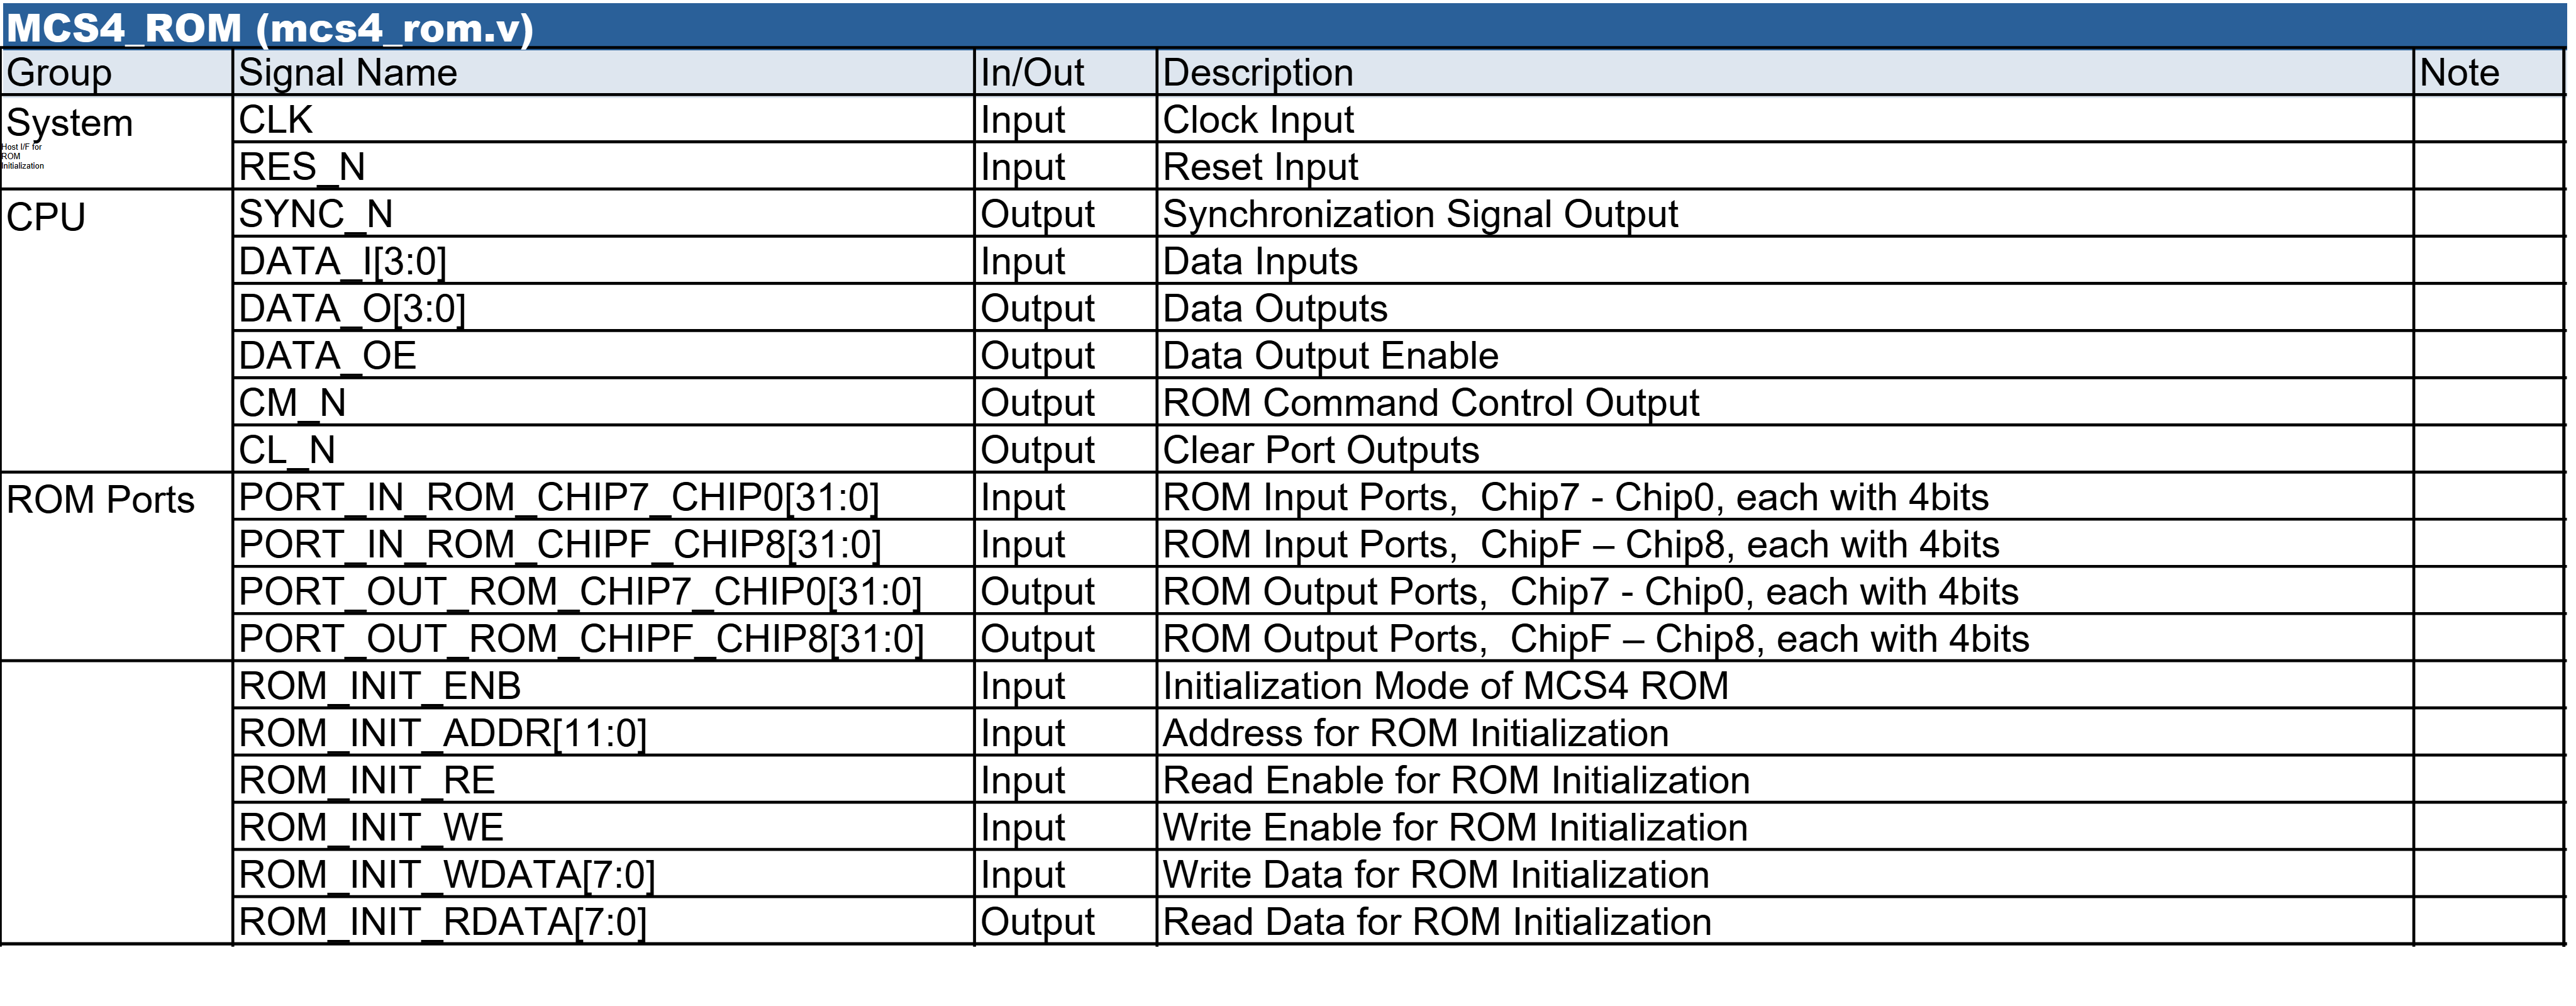
\includegraphics[width=1.00\columnwidth]{./Table/SignalsMCS4ROM.png}
    \caption{I/O Signals of \texttt{MCS4\_ROM}}
    \label{tb:SIGNALSMCS4ROM}
\end{table}
%----------------------------------

%--------------------------------------------------------------
\subsection{\textbf{ROM Initialization}}
After system power-up, ROM contents are initialized using \verb|$readmemh()| with the file \texttt{4001.code} in the \verb|initial| statement, which contains the program code of Busicom's 141-PF calculator using MCS-4 chips.  

The file \texttt{4001.code} can be downloaded from: \\
\url{http://www.4004.com/assets/busicom-141pf-simulator-w-flowchart-071113.zip}

The license of the file is based on: \\
\url{https://creativecommons.org/licenses/by-nc-sa/2.5/legalcode}
\\

For detailed analysis, refer to the disassembled listing: \\
\texttt{Busicom-141PF-Calculator\_asm\_rel-1-0-1.txt}  

Downloadable from: \\
\url{http://www.4004.com/2009/Busicom-141PF-Calculator_asm_rel-1-0-1.txt} 

The license of the file is based on: \\
\url{https://creativecommons.org/licenses/by-nc-sa/2.5/legalcode}


%--------------------------------------------------------------
\subsection{\textbf{ROM Update Procedure}}
ROM content can be modified externally by following manners. \\

\textbf{(1) Method to Write to ROM}\\
\begin{enumerate}
  \item Reset the entire MCS-4 system and halt CPU instruction execution.
  \item Assert the signal \verb|ROM_INIT_ENB|.
  \item Set target address via \verb|ROM_INIT_ADDR[11:0]| and write data via \verb|ROM_INIT_WDATA[7:0]|, then assert \verb|ROM_INIT_WE| for a few clock cycles and deassert.
  \item Repeat for other addresses and data sequentially.
  \item Deassert \verb|ROM_INIT_ENB| after writing.
  \item Release system reset and resume CPU instruction execution.
\end{enumerate}

\textbf{(2) Method to Read from ROM}\\
\begin{enumerate}
  \item Reset the entire MCS-4 system and halt CPU instruction execution.
  \item Assert the signal \verb|ROM_INIT_ENB|.
  \item Set the read address using \verb|ROM_INIT_ADDR[11:0]| and assert \verb|ROM_INIT_RE| for a few clock cycles.
  \item Read data appears on \verb|ROM_INIT_RDATA[7:0]|; then deassert \verb|ROM_INIT_RE|.
  \item Repeat for additional read operations.
  \item Deassert \verb|ROM_INIT_ENB| after completion.
  \item Release system reset and resume CPU instruction execution.
\end{enumerate}

\textit{Note: Read operations may immediately follow write operations while ROM\_INIT\_ENB remains asserted.}

%--------------------------------------------------------------
\subsection{\textbf{Implementation of \texttt{4001} I/O Ports}}
On actual \texttt{4001} chips, the directionality of I/O ports is fixed via metal options.  
In this system, both input and output ports are usable simultaneously.  
Signals are separated into independent input and output paths.  
Write operations affect the output port, while read operations retrieve the logic level of the input port.  
Figure~\ref{fig:METALOPTIONMCS4ROM} illustrates the assumed metal option settings.

%----------------------------------
\begin{table}[htbp]
    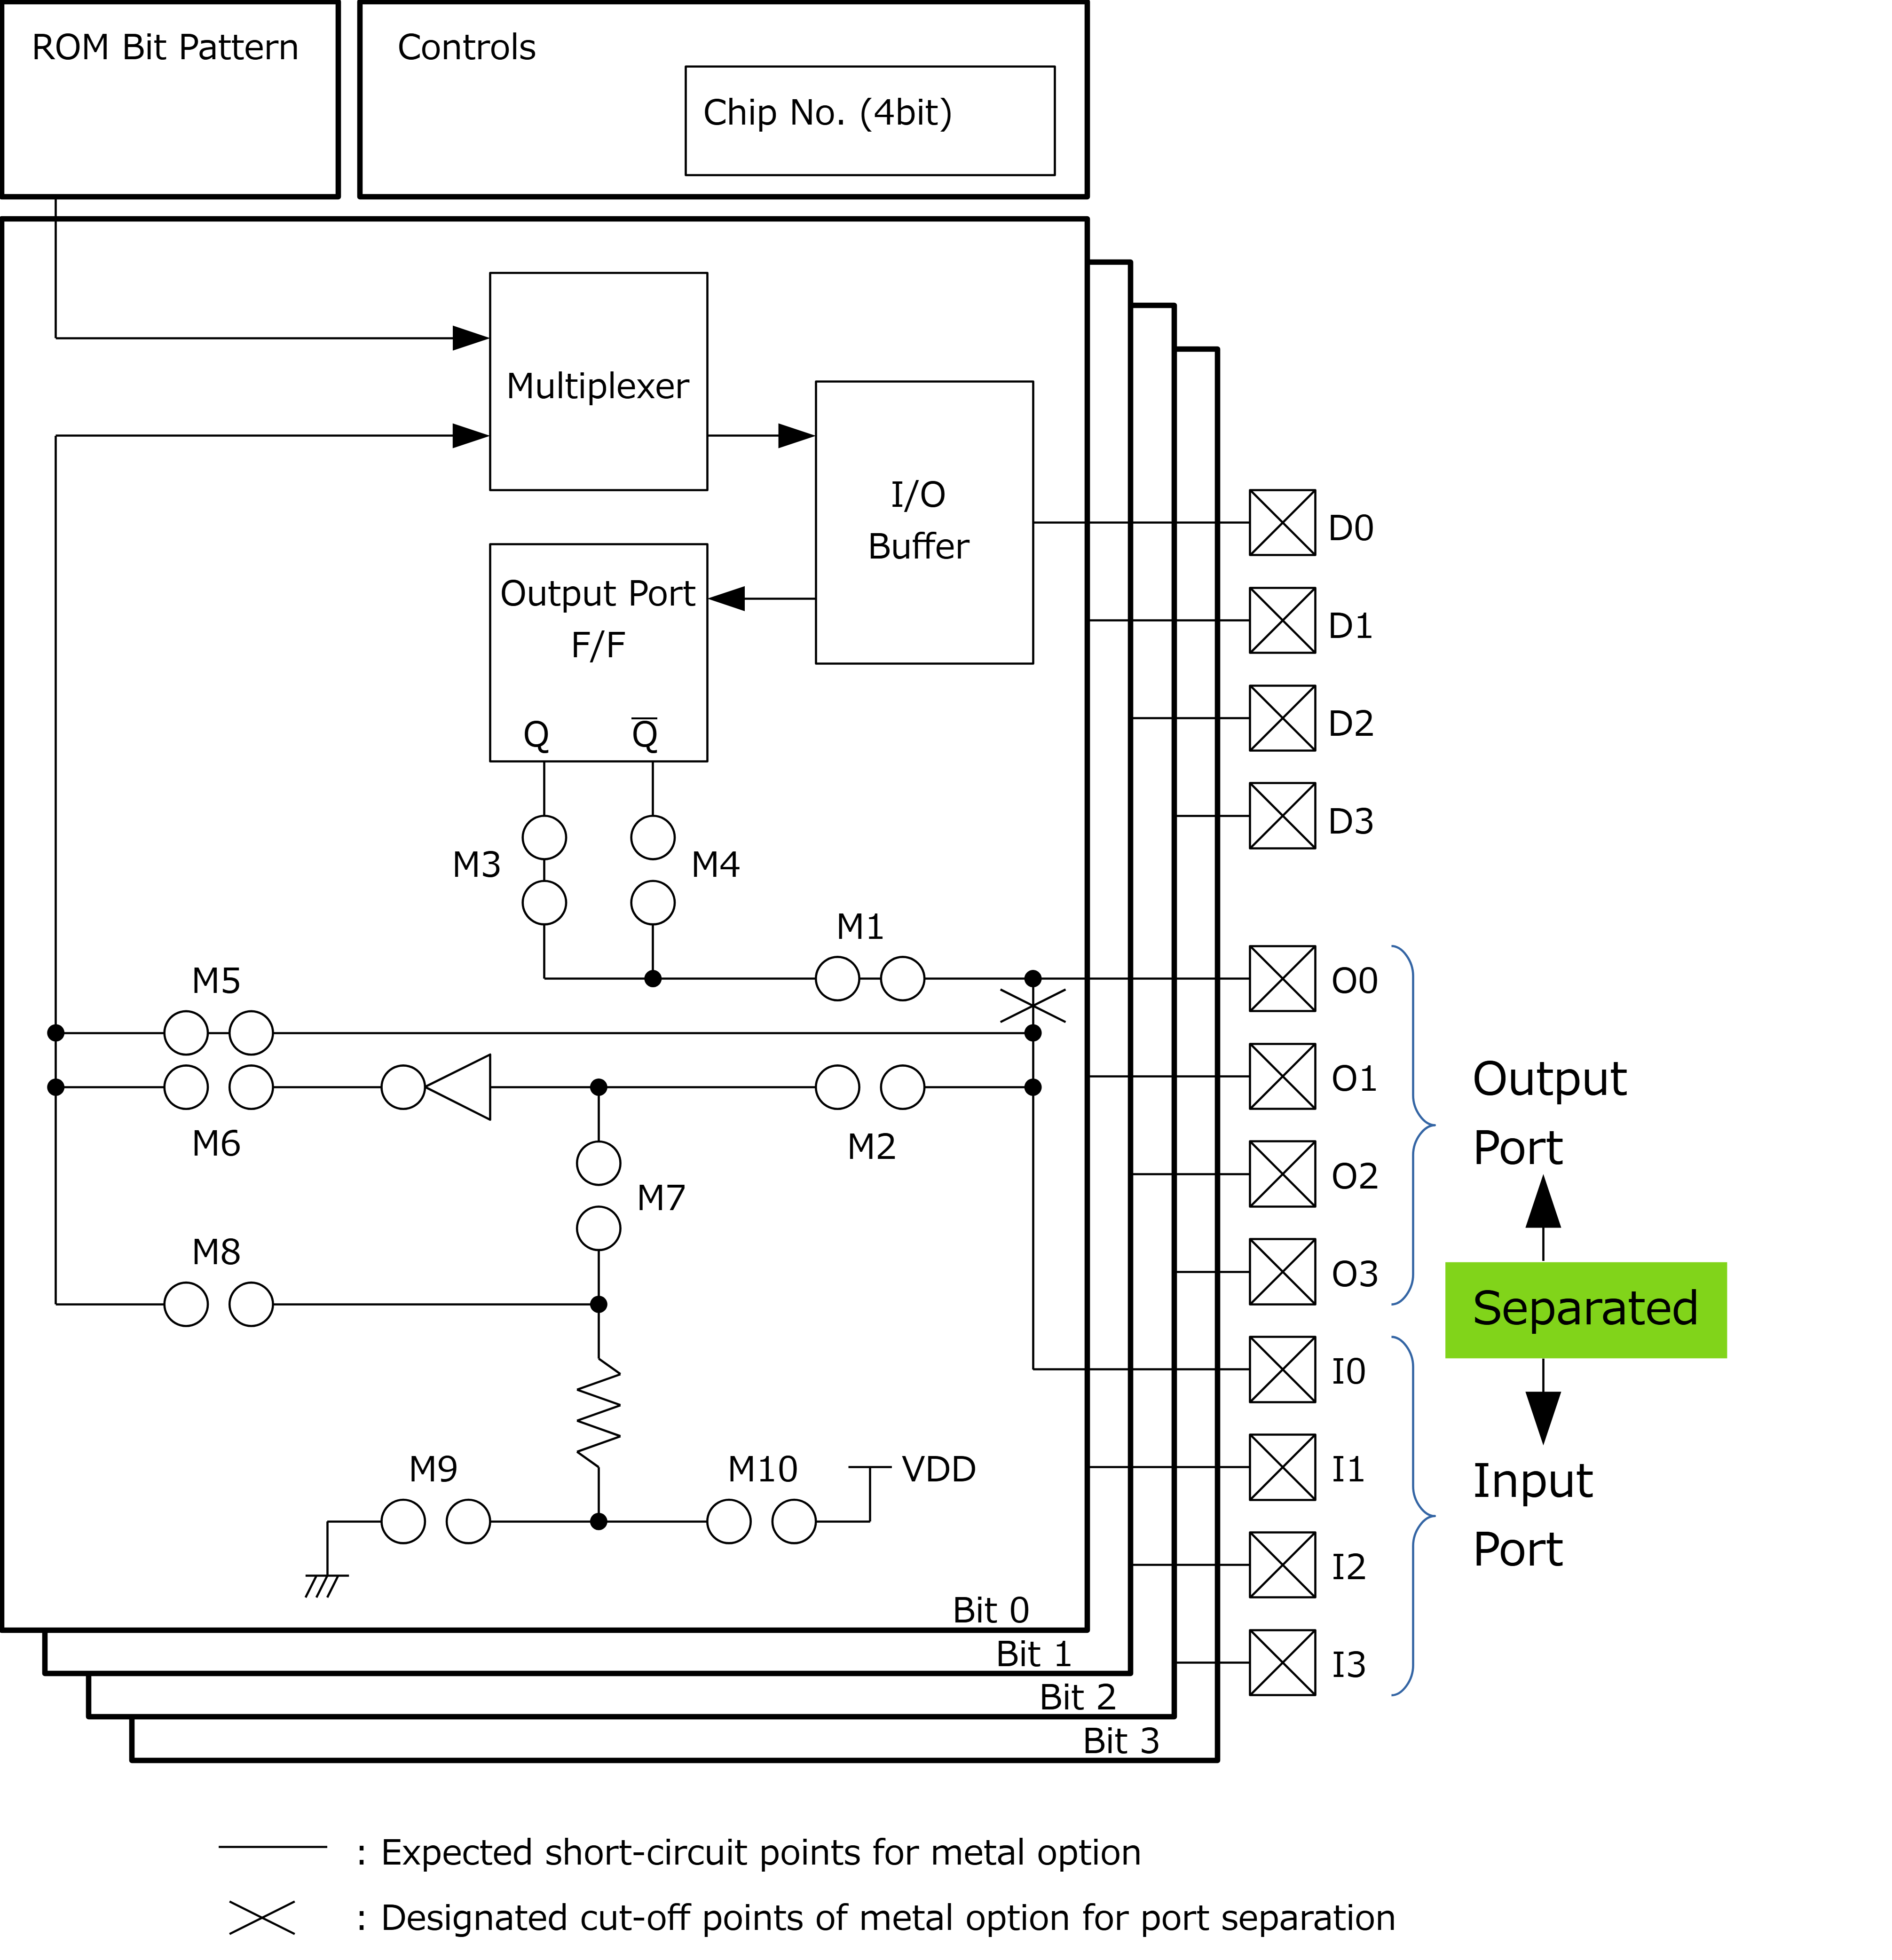
\includegraphics[width=0.66\columnwidth]{./Figure/MCS4ROMMetalOption.png}
    \caption{Assumed Metal Option Settings in \texttt{MCS4\_ROM}}
    \label{fig:METALOPTIONMCS4ROM}
\end{table}
%----------------------------------

The I/O port signals for the \texttt{MCS4\_ROM} module are formed by concatenating those from multiple \texttt{4001} chips:

\begin{itemize}
  \item \verb|PORT_IN_ROM_CHIP7_CHIP0[31:0]| — Input ports from chips 7 through 0
  \item \verb|PORT_IN_ROM_CHIPF_CHIP8[31:0]| — Input ports from chips 15 through 8
  \item \verb|PORT_OUT_ROM_CHIP7_CHIP0[31:0]| — Output ports from chips 7 through 0
  \item \verb|PORT_OUT_ROM_CHIPF_CHIP8[31:0]| — Output ports from chips 15 through 8
\end{itemize}

%--------------------------------------------------------------
\subsection{\textbf{RTL Contents of the \texttt{MCS4\_ROM} Module}}
The RTL code \texttt{mcs4\_rom.v} includes the ROM memory, input ports, and output ports for all 16 \texttt{4001} chips.  

The module operates in synchronization with the CPU.

During instruction fetch and the second cycle of the \texttt{FIN} instruction,  
address is captured in states A1–A3 and read data is output during states M1–M2.

When executing the \texttt{SRC} instruction, the signal \verb|CM_ROM_N| is asserted in state X2, prompting retrieval of the SRC address.

If the upper 4 bits of the instruction code (\texttt{OPR}) fetched in state M2 equal \verb|4'b1110| (indicating data access operations), then \verb|CM_ROM_N| is asserted again in the subsequent M2 state.  
The lower 4 bits (\texttt{OPA}) on the data bus are decoded to determine the target and direction (read/write), and the specified read or write operation is executed in state X2.

%==============================================================
\section{Logic of the \texttt{MCS4\_RAM} Module (4002)}
%--------------------------------------------------------------
\subsection{\textbf{Module \texttt{MCS4\_RAM} Incorporates 32 \texttt{4002} (RAM) Chips}}
The module \texttt{MCS4\_RAM} consists of a block comprising 32 chips of \texttt{4002} (RAM); 8 banks x 4chips; totaling 2560 nibbles (1280 bytes).
The RTL implementation is defined in \texttt{mcs4\_ram.v}.  
Table~\ref{tb:SIGNALSMCS4RAM} presents the input/output signals of the \texttt{MCS4\_RAM} module.

%----------------------------------
\begin{table}[htbp]
    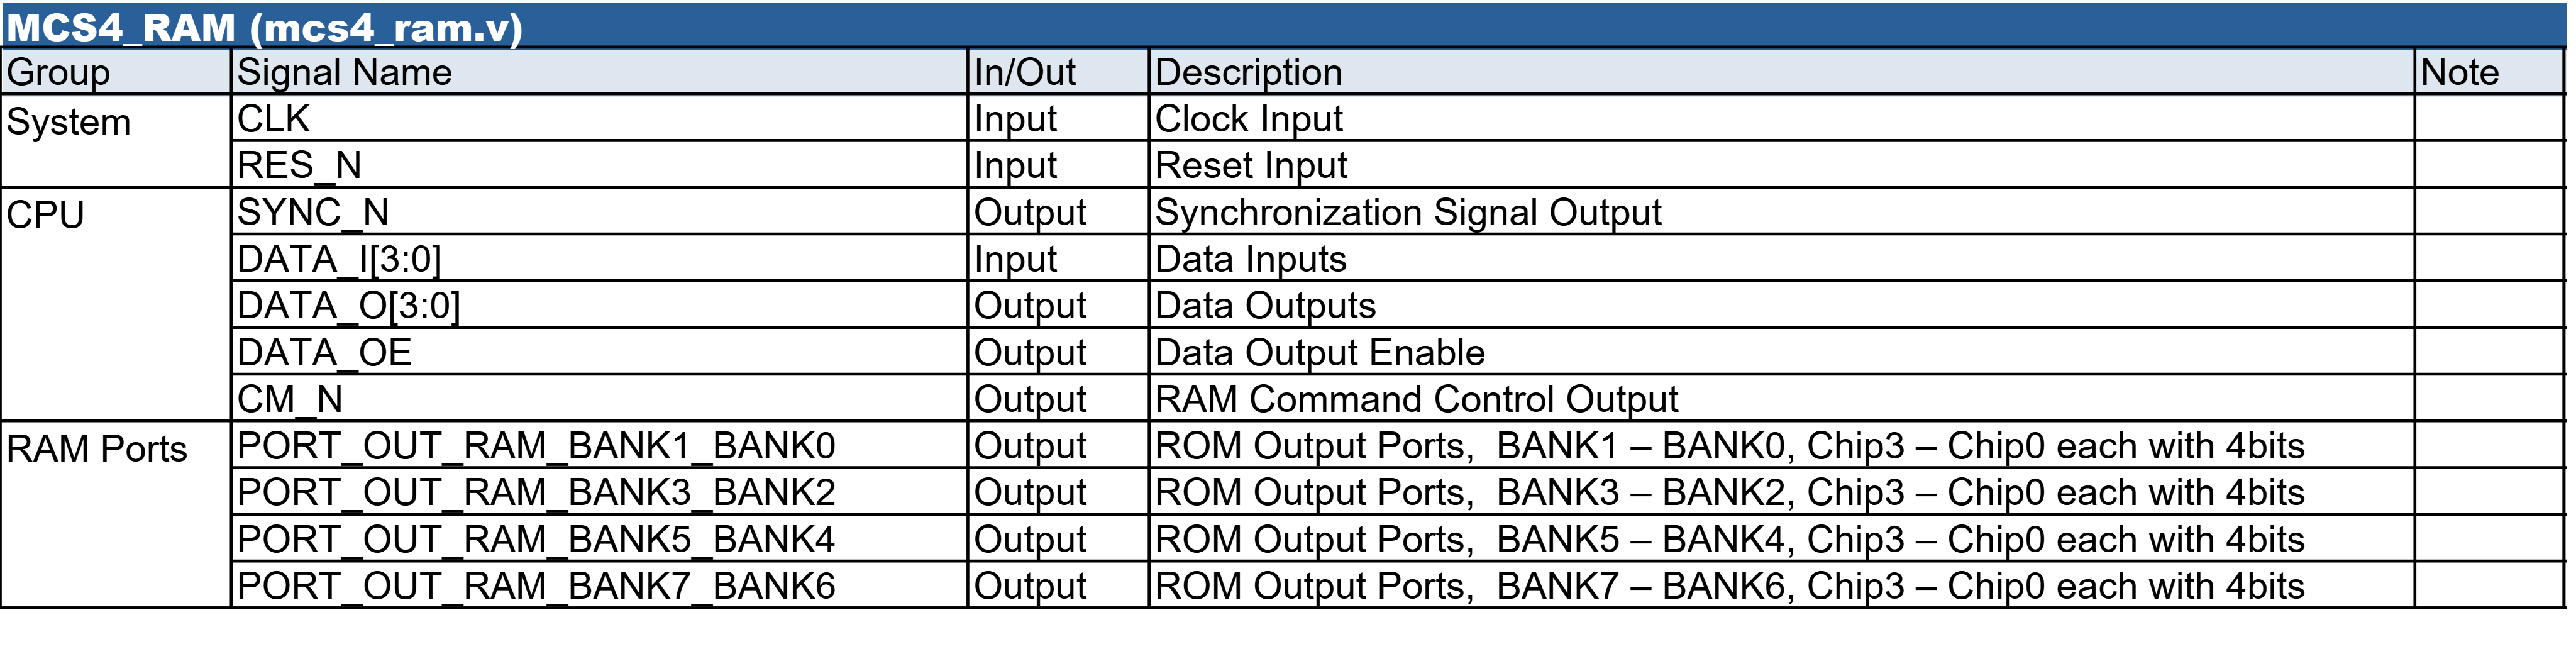
\includegraphics[width=1.00\columnwidth]{./Table/SignalsMCS4RAM.png}
    \caption{I/O Signals of \texttt{MCS4\_RAM}}
    \label{tb:SIGNALSMCS4RAM}
\end{table}
%----------------------------------

%--------------------------------------------------------------
\subsection{Expansion of RAM Banks}
The 4004 CPU outputs four signals: \verb|CM_RAM_N[3:0]|.  
If these are used as one-hot signals directly without external circuitry, the system can support up to four RAM banks. However, by encoding \verb|CM_RAM_N[3:0]| and decoding them inside the module, the number of RAM banks can be expanded to eight. 
In the \texttt{MCS4\_RAM} module, \verb|CM_RAM_N[3:0]| from the CPU is decoded to generate eight bank-select signals as shown in Table~\ref{tb:DECODECMRAMN}.

%----------------------------------
\begin{table}[htbp]
    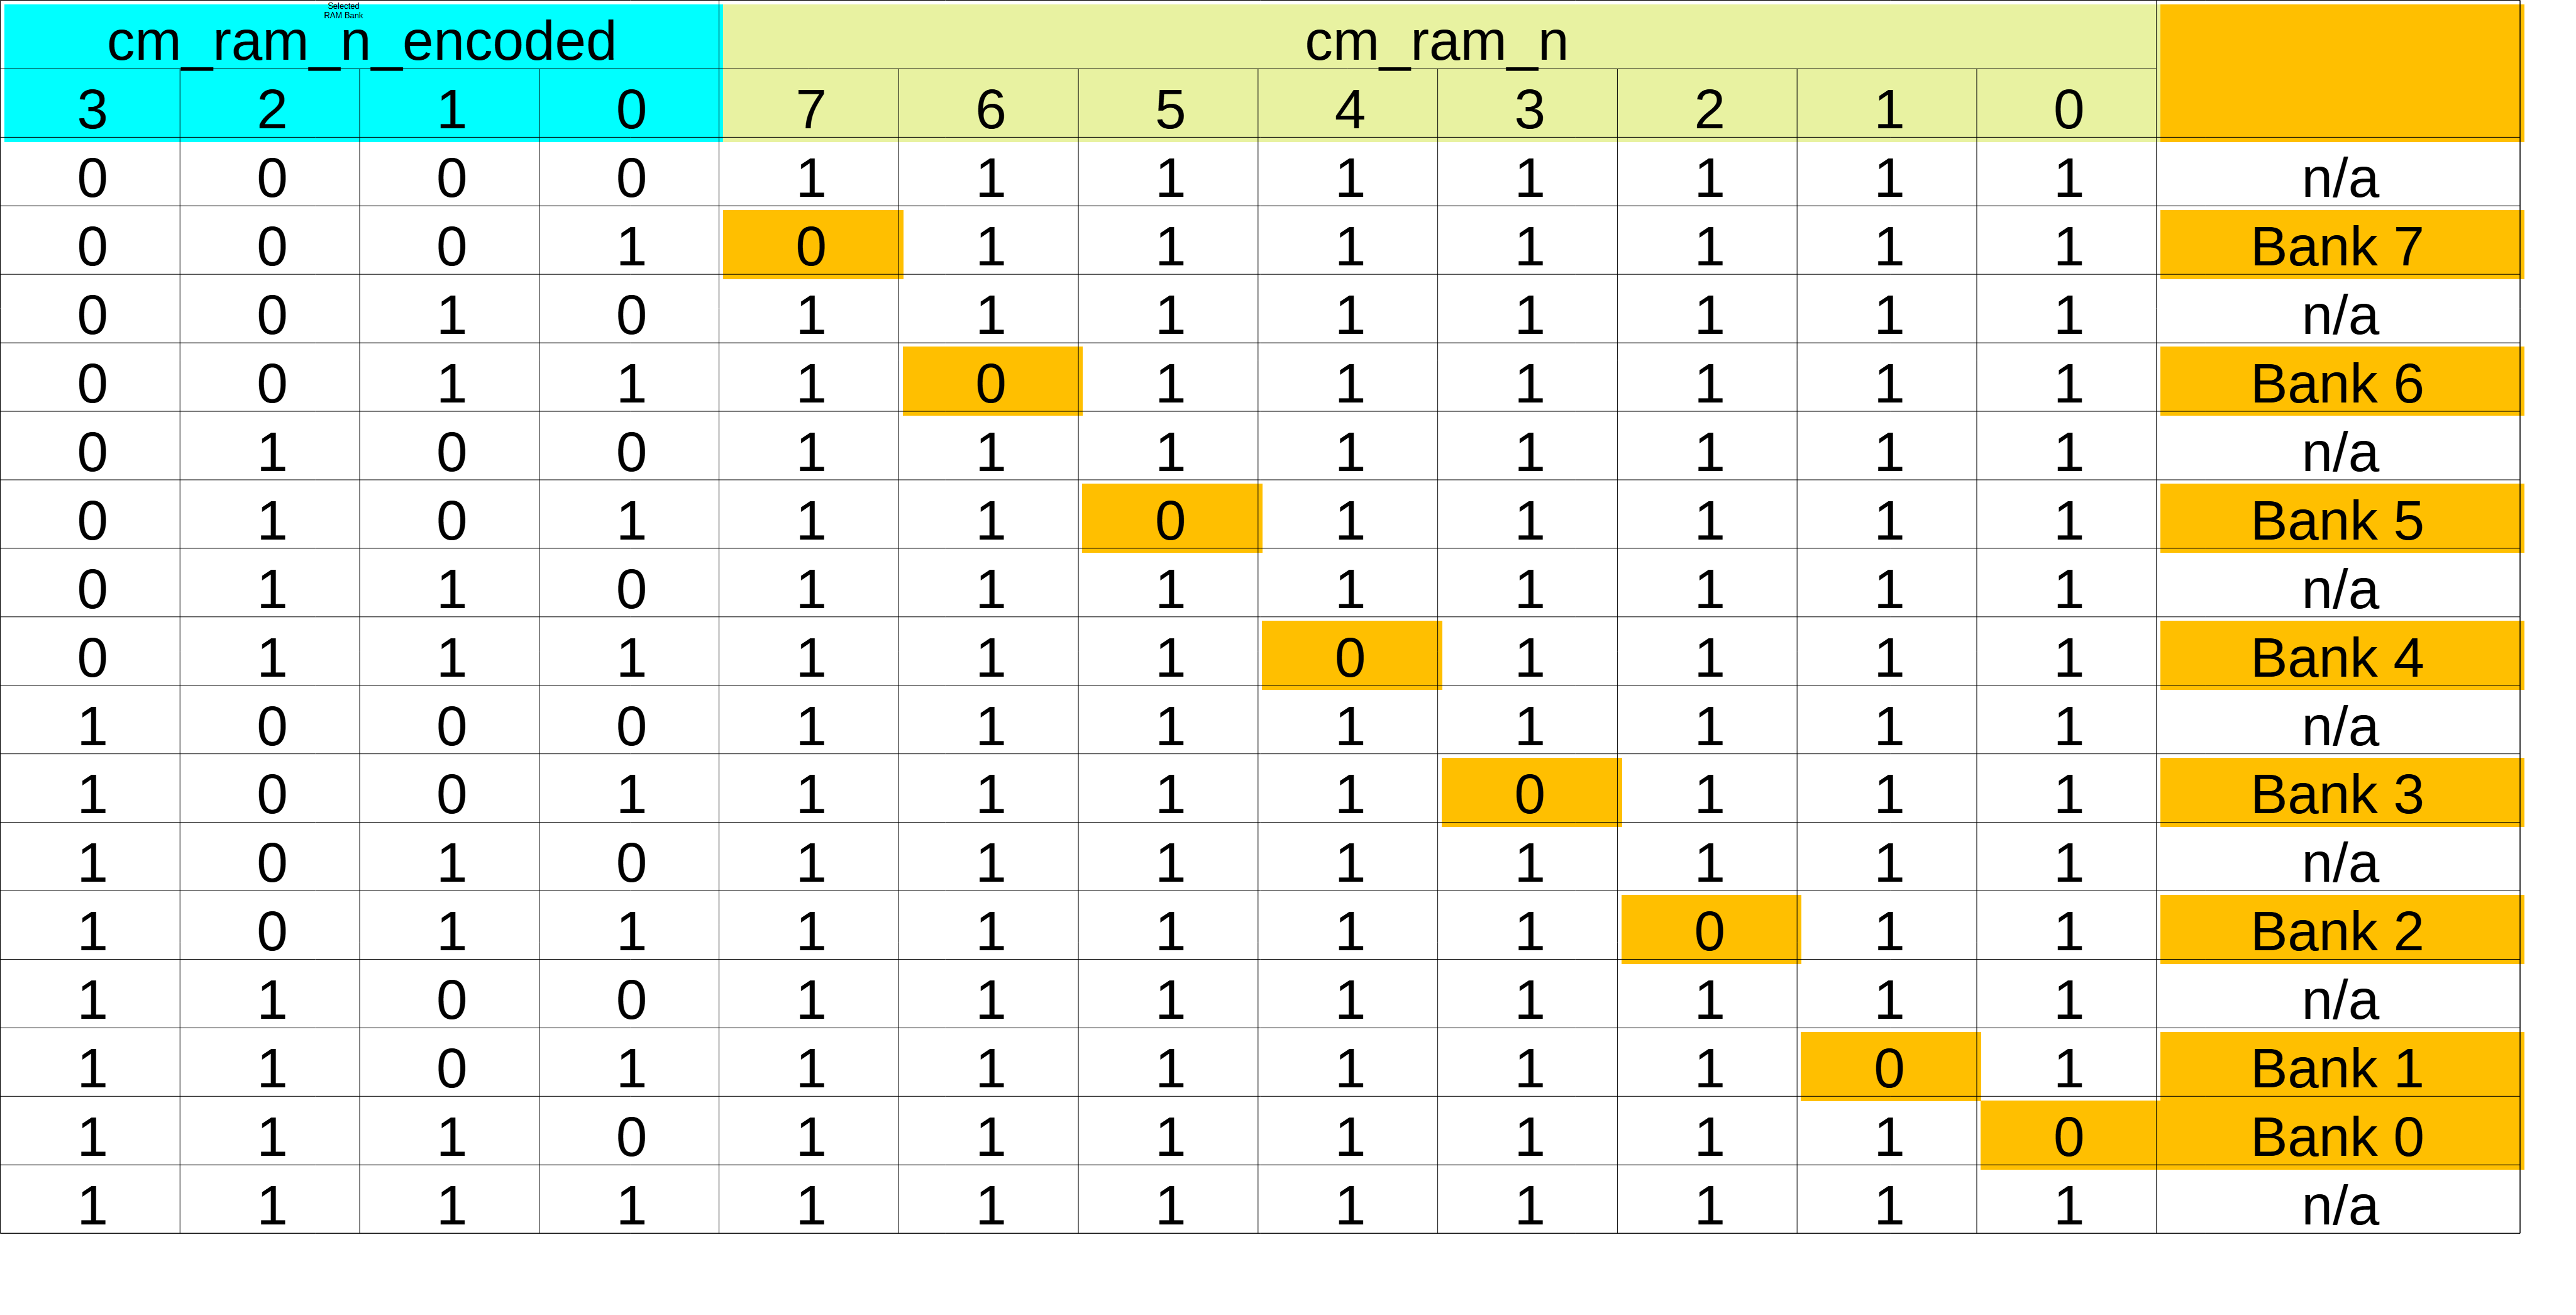
\includegraphics[width=1.00\columnwidth]{./Table/DecodeCMRAM.png}
    \caption{Decode of CM\_RAM\_N[3:0]}
    \label{tb:DECODECMRAMN}
\end{table}
%----------------------------------

%--------------------------------------------------------------
\subsection{\textbf{Implementation of \texttt{4002} Output Ports}}
The output port signals for the \texttt{MCS4\_RAM} module are formed by concatenating those from multiple \texttt{4002} chips:

\begin{itemize}
  \item \verb|PORT_OUT_RAM_BANK1_BANK0[31:0]| — Output ports BANK1/Chip3-Chip0, and  BANK0/Chip3-Chip0
  \item \verb|PORT_OUT_RAM_BANK3_BANK2[31:0]| — Output ports BANK3/Chip3-Chip0, and  BANK2/Chip3-Chip0
  \item \verb|PORT_OUT_RAM_BANK5_BANK4[31:0]| — Output ports BANK5/Chip3-Chip0, and  BANK4/Chip3-Chip0
  \item \verb|PORT_OUT_RAM_BANK7_BANK6[31:0]| — Output ports BANK7/Chip3-Chip0, and  BANK6/Chip3-Chip0
\end{itemize}

%--------------------------------------------------------------
\subsection{\textbf{RTL Contents of the \texttt{MCS4\_RAM} Module}}
The RTL code in \texttt{mcs4\_ram.v} describes the memory and output ports for 8 banks × 4 chips of \texttt{4002} RAM.  

The module operates in synchronization with the CPU.

When the CPU executes the \texttt{SRC} instruction, \verb|CM_RAM_N[3:0]| is asserted during state X2,  
which triggers the loading of the SRC address.

During state M2, the CPU fetches the upper 4 bits (\texttt{OPR}) of the instruction code.  
If \texttt{OPR} matches the data-access opcode (\verb|4'b1110|), then \verb|CM_RAM_N[3:0]| is asserted in the following M2 cycle.  
The lower 4 bits (\texttt{OPA}) on the data bus are decoded to determine the access target and operation direction (read/write), and the corresponding read or write operation is performed during state X2.

%--------------------------------------------------------------
\subsection{Module Structure of \texttt{MCS4\_RAM}}
Within the \texttt{MCS4\_RAM} module, a total of 32 instances of the \texttt{MCS4\_RAM\_CHIP} module—each representing one \texttt{4002} RAM chip—are instantiated.  
The \texttt{MCS4\_RAM\_CHIP} module itself is also defined within the RTL code \texttt{mcs4\_ram.v}.  
Each RAM bank consists of four \texttt{MCS4\_RAM\_CHIP} instances, and these must be distinguished by their chip number.

To identify each chip, two input signals—\texttt{P0} and \texttt{P1}—are provided to the \texttt{MCS4\_RAM\_CHIP} module:
\begin{itemize}
  \item \texttt{P0}: A chip select signal found in actual \texttt{4002} devices.
  \item \texttt{P1}: A signal introduced to distinguish between chip types (e.g., \texttt{4002-1} and \texttt{4002-2}) at the input level.
\end{itemize}

When instantiating \texttt{MCS4\_RAM\_CHIP} modules within \texttt{MCS4\_RAM}, the logic level of \texttt{P0} and \texttt{P1} is explicitly assigned.

%--------------------------------------------------------------
\subsection{Reset Behavior and RAM Initialization}
Real \texttt{4002} chips feature an internal mechanism to initialize RAM contents to zero during reset.  
In actual devices, asserting the reset signal for 32 instruction cycles (equivalent to 256 system clock cycles) triggers an internal counter to clear the RAM contents.

This behavior is replicated in the current system.  
The \texttt{MCS4\_RAM\_CHIP} module incorporates similar logic such that asserting the reset signal \texttt{RES\_N} for 64 or more system clock cycles initializes RAM contents to zero.

Unlike modern RAM devices—which generally lack hardware-level zero-clear functionality—the \texttt{4002} RAM's automatic initialization eliminates the need for memory-clear routines in software, contributing to reduced program size.

%==============================================================
%==============================================================
\section{Logic of the \texttt{MCS4\_SHIFTER} Module (4003)}
%--------------------------------------------------------------
\subsection{Simple Shift Register \texttt{4003} (Shift Register) Chip}
The \texttt{MCS4\_SHIFTER} module implements the functionality of the \texttt{4003} chip, which serves as a serial-in/parallel-out shift register. Its RTL description is defined in the file \texttt{mcs4\_shifter.v}.
Table~\ref{tb:SIGNALSMCS4SHIFTER} presents the input/output signals of the \texttt{MCS4\_SHIFTER} module.

%----------------------------------
\begin{table}[htbp]
    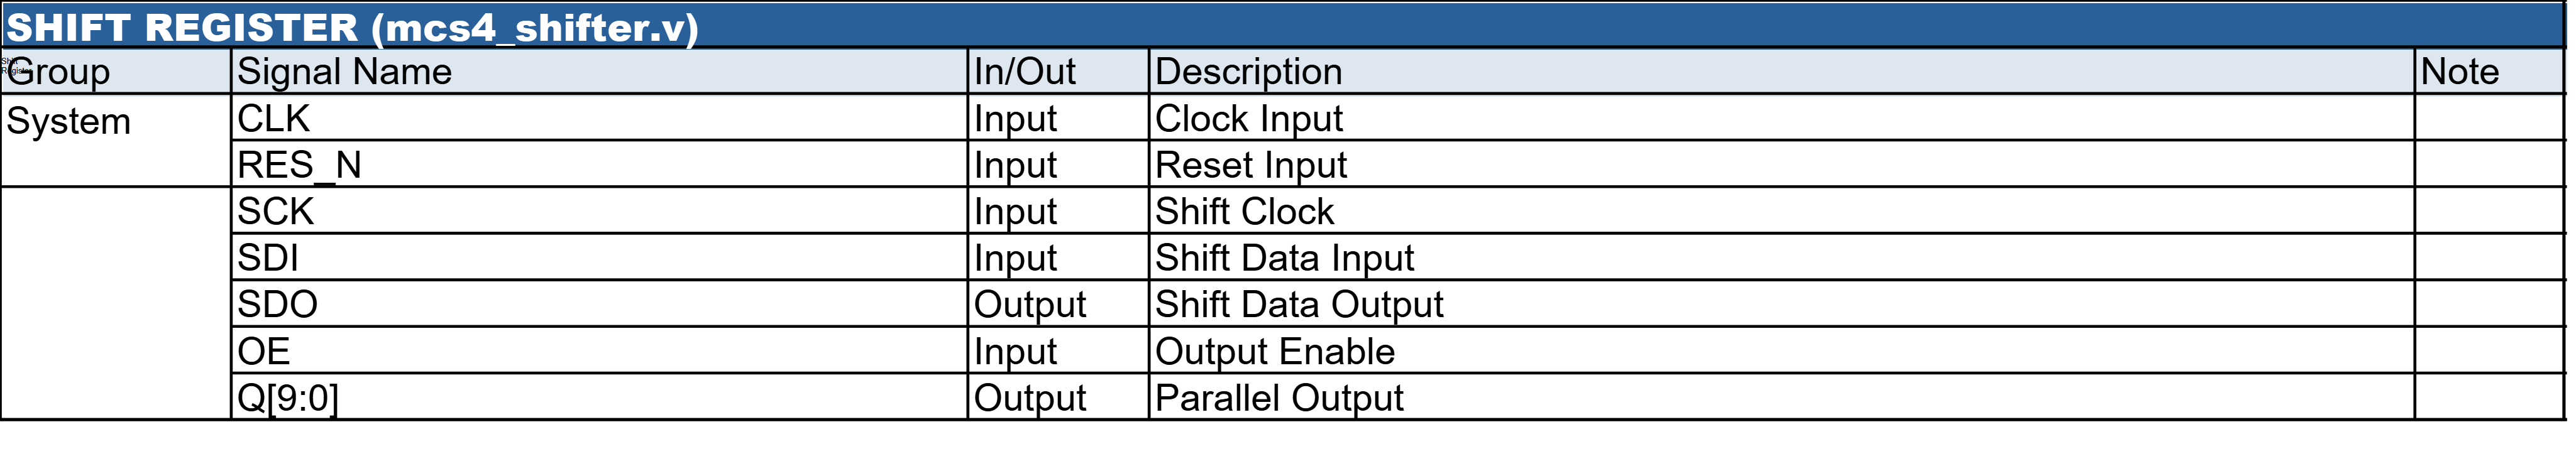
\includegraphics[width=1.00\columnwidth]{./Table/SignalsMCS4SHIFTER.png}
    \caption{I/O Signals of \texttt{MCS4\_SHIFTER}}
    \label{tb:SIGNALSMCS4SHIFTER}
\end{table}
%----------------------------------

%--------------------------------------------------------------
\subsection{\textbf{RTL Contents of the \texttt{MCS4\_SHIFTER} Module}}
The RTL module \texttt{mcs4\_shifter.v} implements a 10-bit shift register.  
Data is shifted into the register on the rising edge of the serial clock signal \texttt{SCK} from the serial data input \texttt{SDI}, and shifted out via the serial data output \texttt{SDO}.

The module features an output enable signal \texttt{OE}, which determines the behavior of the parallel output \texttt{Q[9:0]}:
\begin{itemize}
  \item If \texttt{OE} is \texttt{High}, the contents of the 10-bit shift register are presented at \texttt{Q[9:0]}.
  \item If \texttt{OE} is \texttt{Low}, the output \texttt{Q[9:0]} is forced to zero.
\end{itemize}

%==============================================================
